This project involves the modelling, simulation, control system design, and implementation of a rider-less, self-balancing bicycle. Bicycles and their stability properties have been studied for well over a century, most notably by academics such as Whipple (1899, \cite{whipple}), Papadopoulos (1980s onwards, \cite{papadopoulos}), and Astrom (2005, \cite{astrom}). Most individuals know that a bicycle can be self-stable under certain conditions but it is still commonly unclear what primarily contributes to this self-stability. The full form of the equations of motion do not aid the intuitive understanding of bicycle stability and dynamics, as they are a set of coupled and highly non-linear differential equations. Thus, simplifying assumptions must be sought out. \\

\noindent In addition to simply understanding the causes of self-stability of a bicycle, there are further considerations to studying a bicycle in the frameworks of dynamics and control theory. For example, how does a human stabilise a bicycle and is it possible to replicate this behaviour with motors? What makes a bike more or less stable (for instance, changes in geometry, mass distribution, or wheel size - to name a few)? And would there be a benefit in having an \textit{assisted} bicycle for certain people in certain situations? \\

\noindent This project therefore aims to try and answer - at least in part - some of these questions, with a primary focus on designing suitable control systems that achieve closed-loop stability over a large range of forward velocities. \\

Finally, the report details the implementation of the designed control laws for two rider-less bicycles. Firstly, a \textit{Lego Mindstorms} prototype and secondly a full-scale, adult bicycle. Both bicycles are depicted in Figures \ref{fig:lego} and \ref{fig:fs} below. These bicycles however only have a drive actuator, to provide forward velocity, and an actuator placed at the handlebars to provide a \textit{steer} torque. Without the additional component of being able to provide a \textit{lean} torque, it is extremely difficult to guarantee stability at near-zero forward speed, as will be shown in this report. The bicycles being studied in this case can therefore be classed as \textit{underactuated systems}.

\begin{figure}[H]
\centering
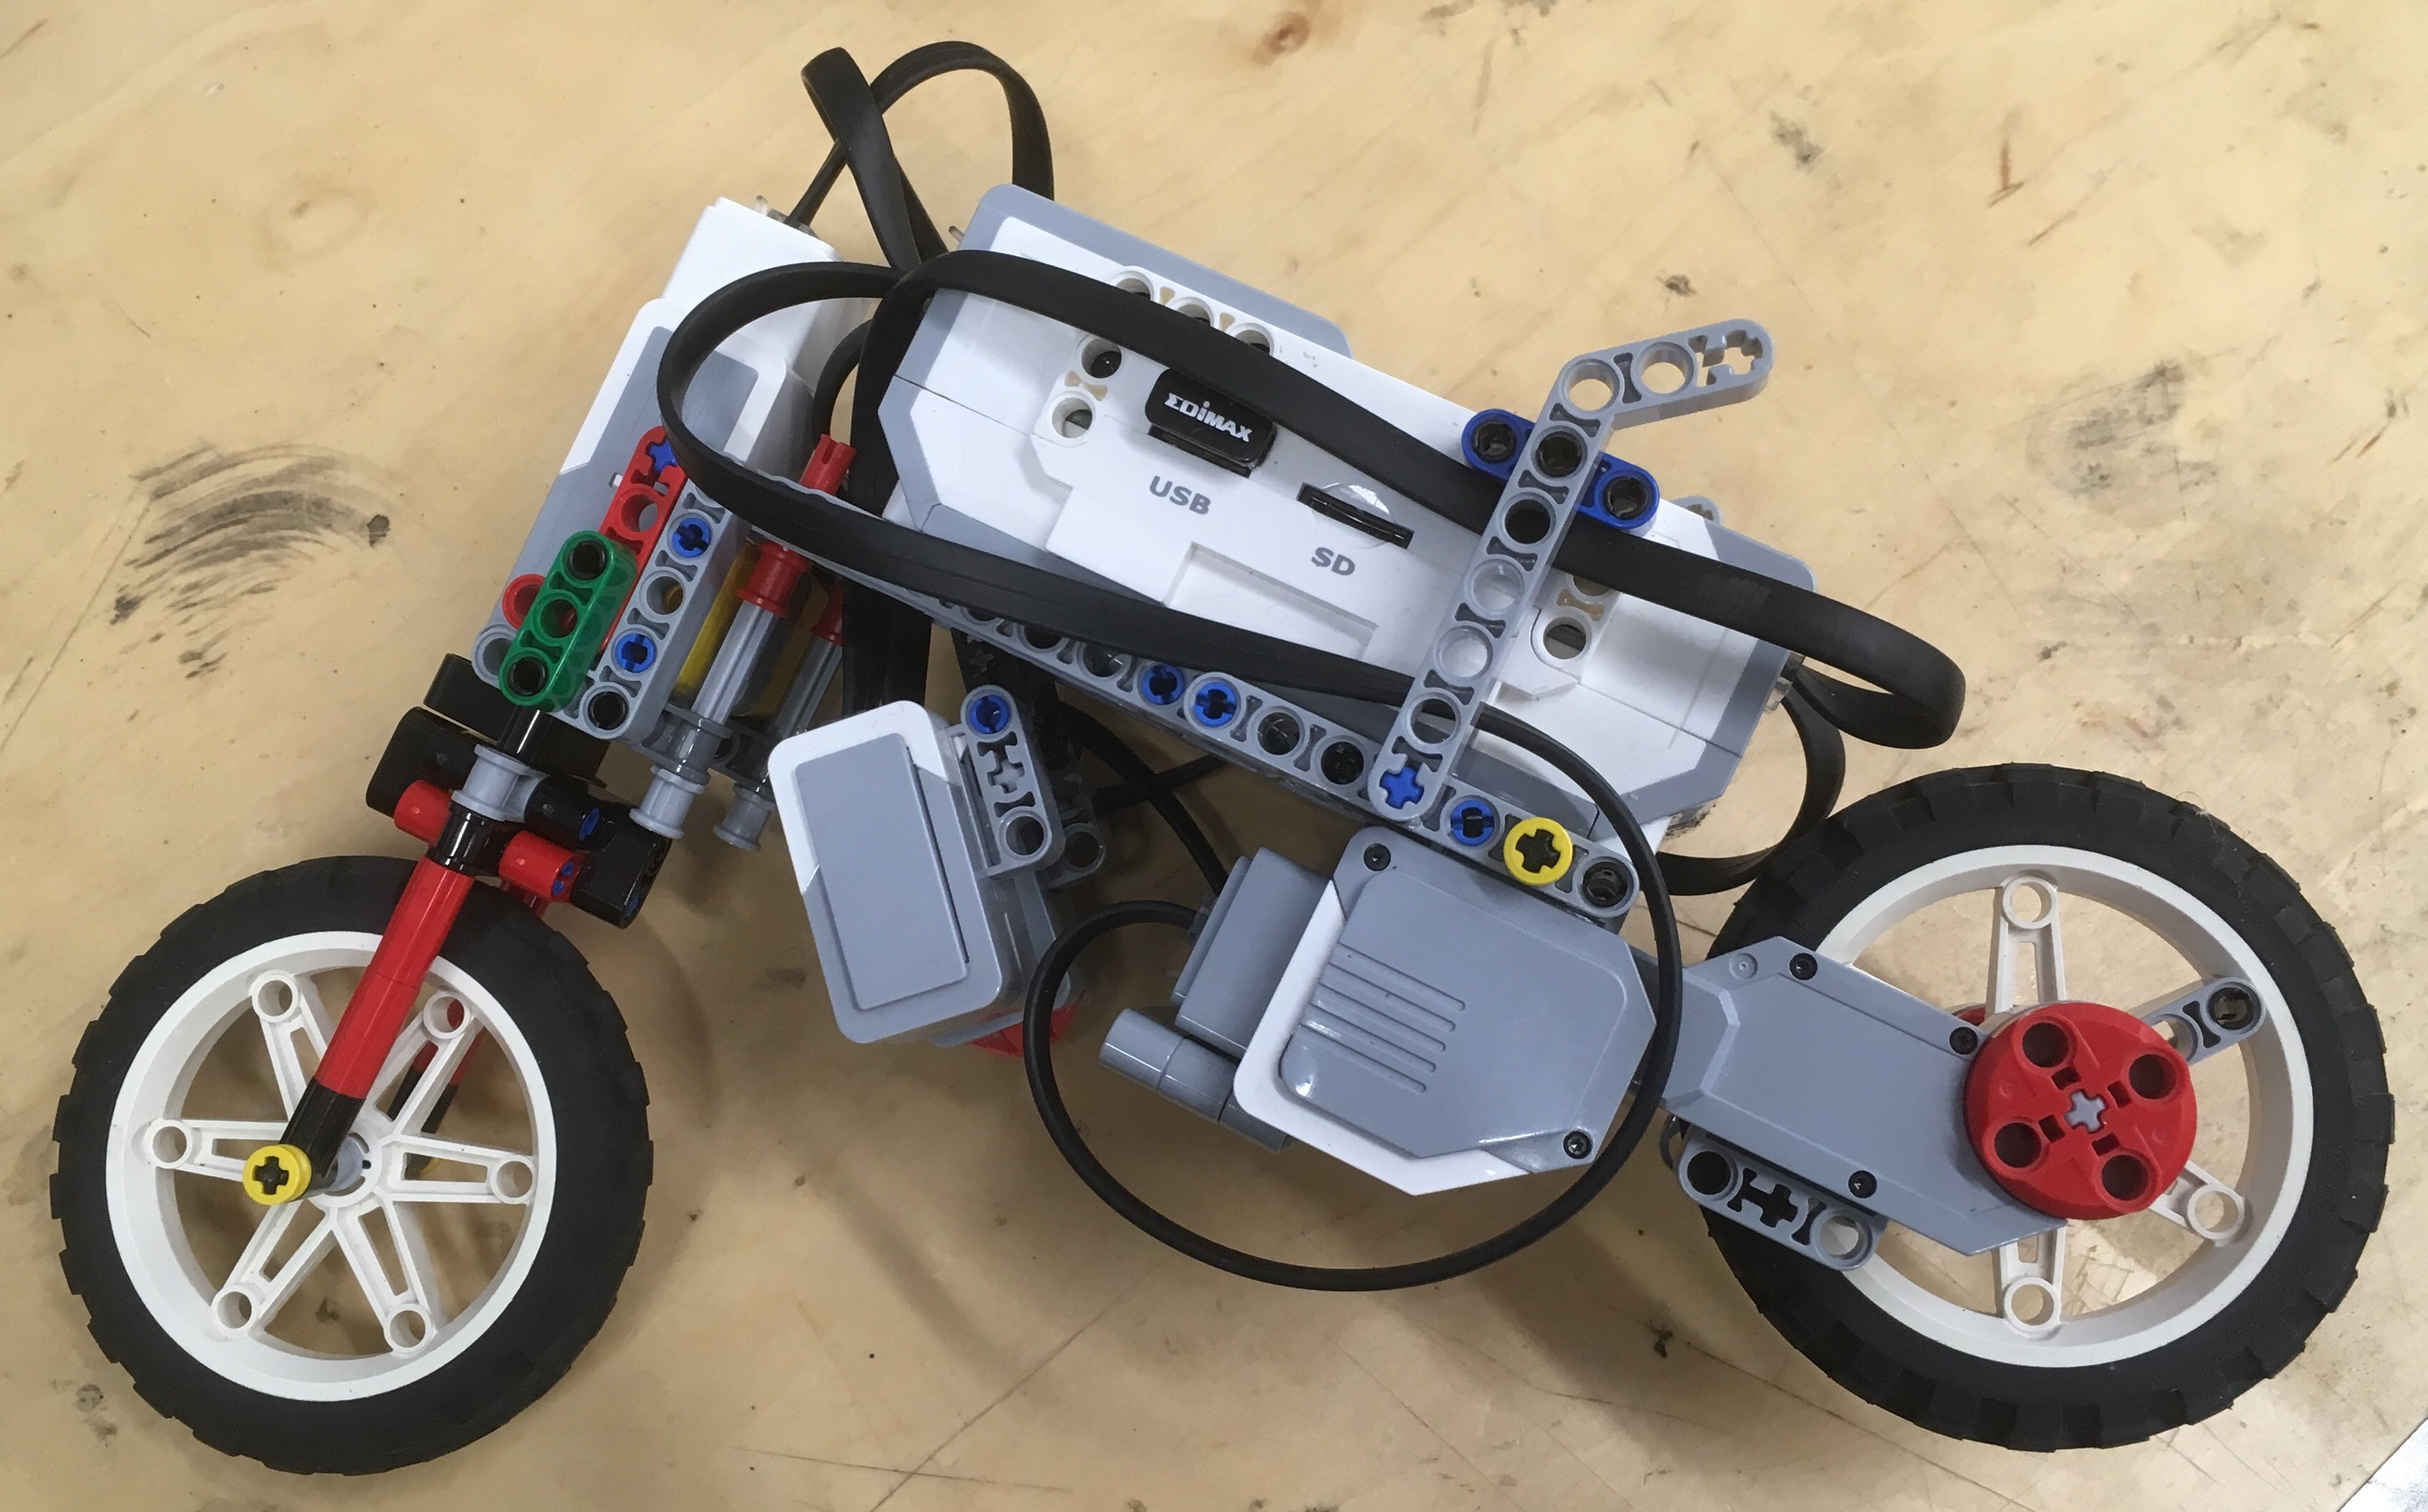
\includegraphics[scale=0.085]{LegoBike.jpg}
\caption{Lego Prototype Bicycle}
\label{fig:lego}
\end{figure}

\begin{figure}[H]
\centering
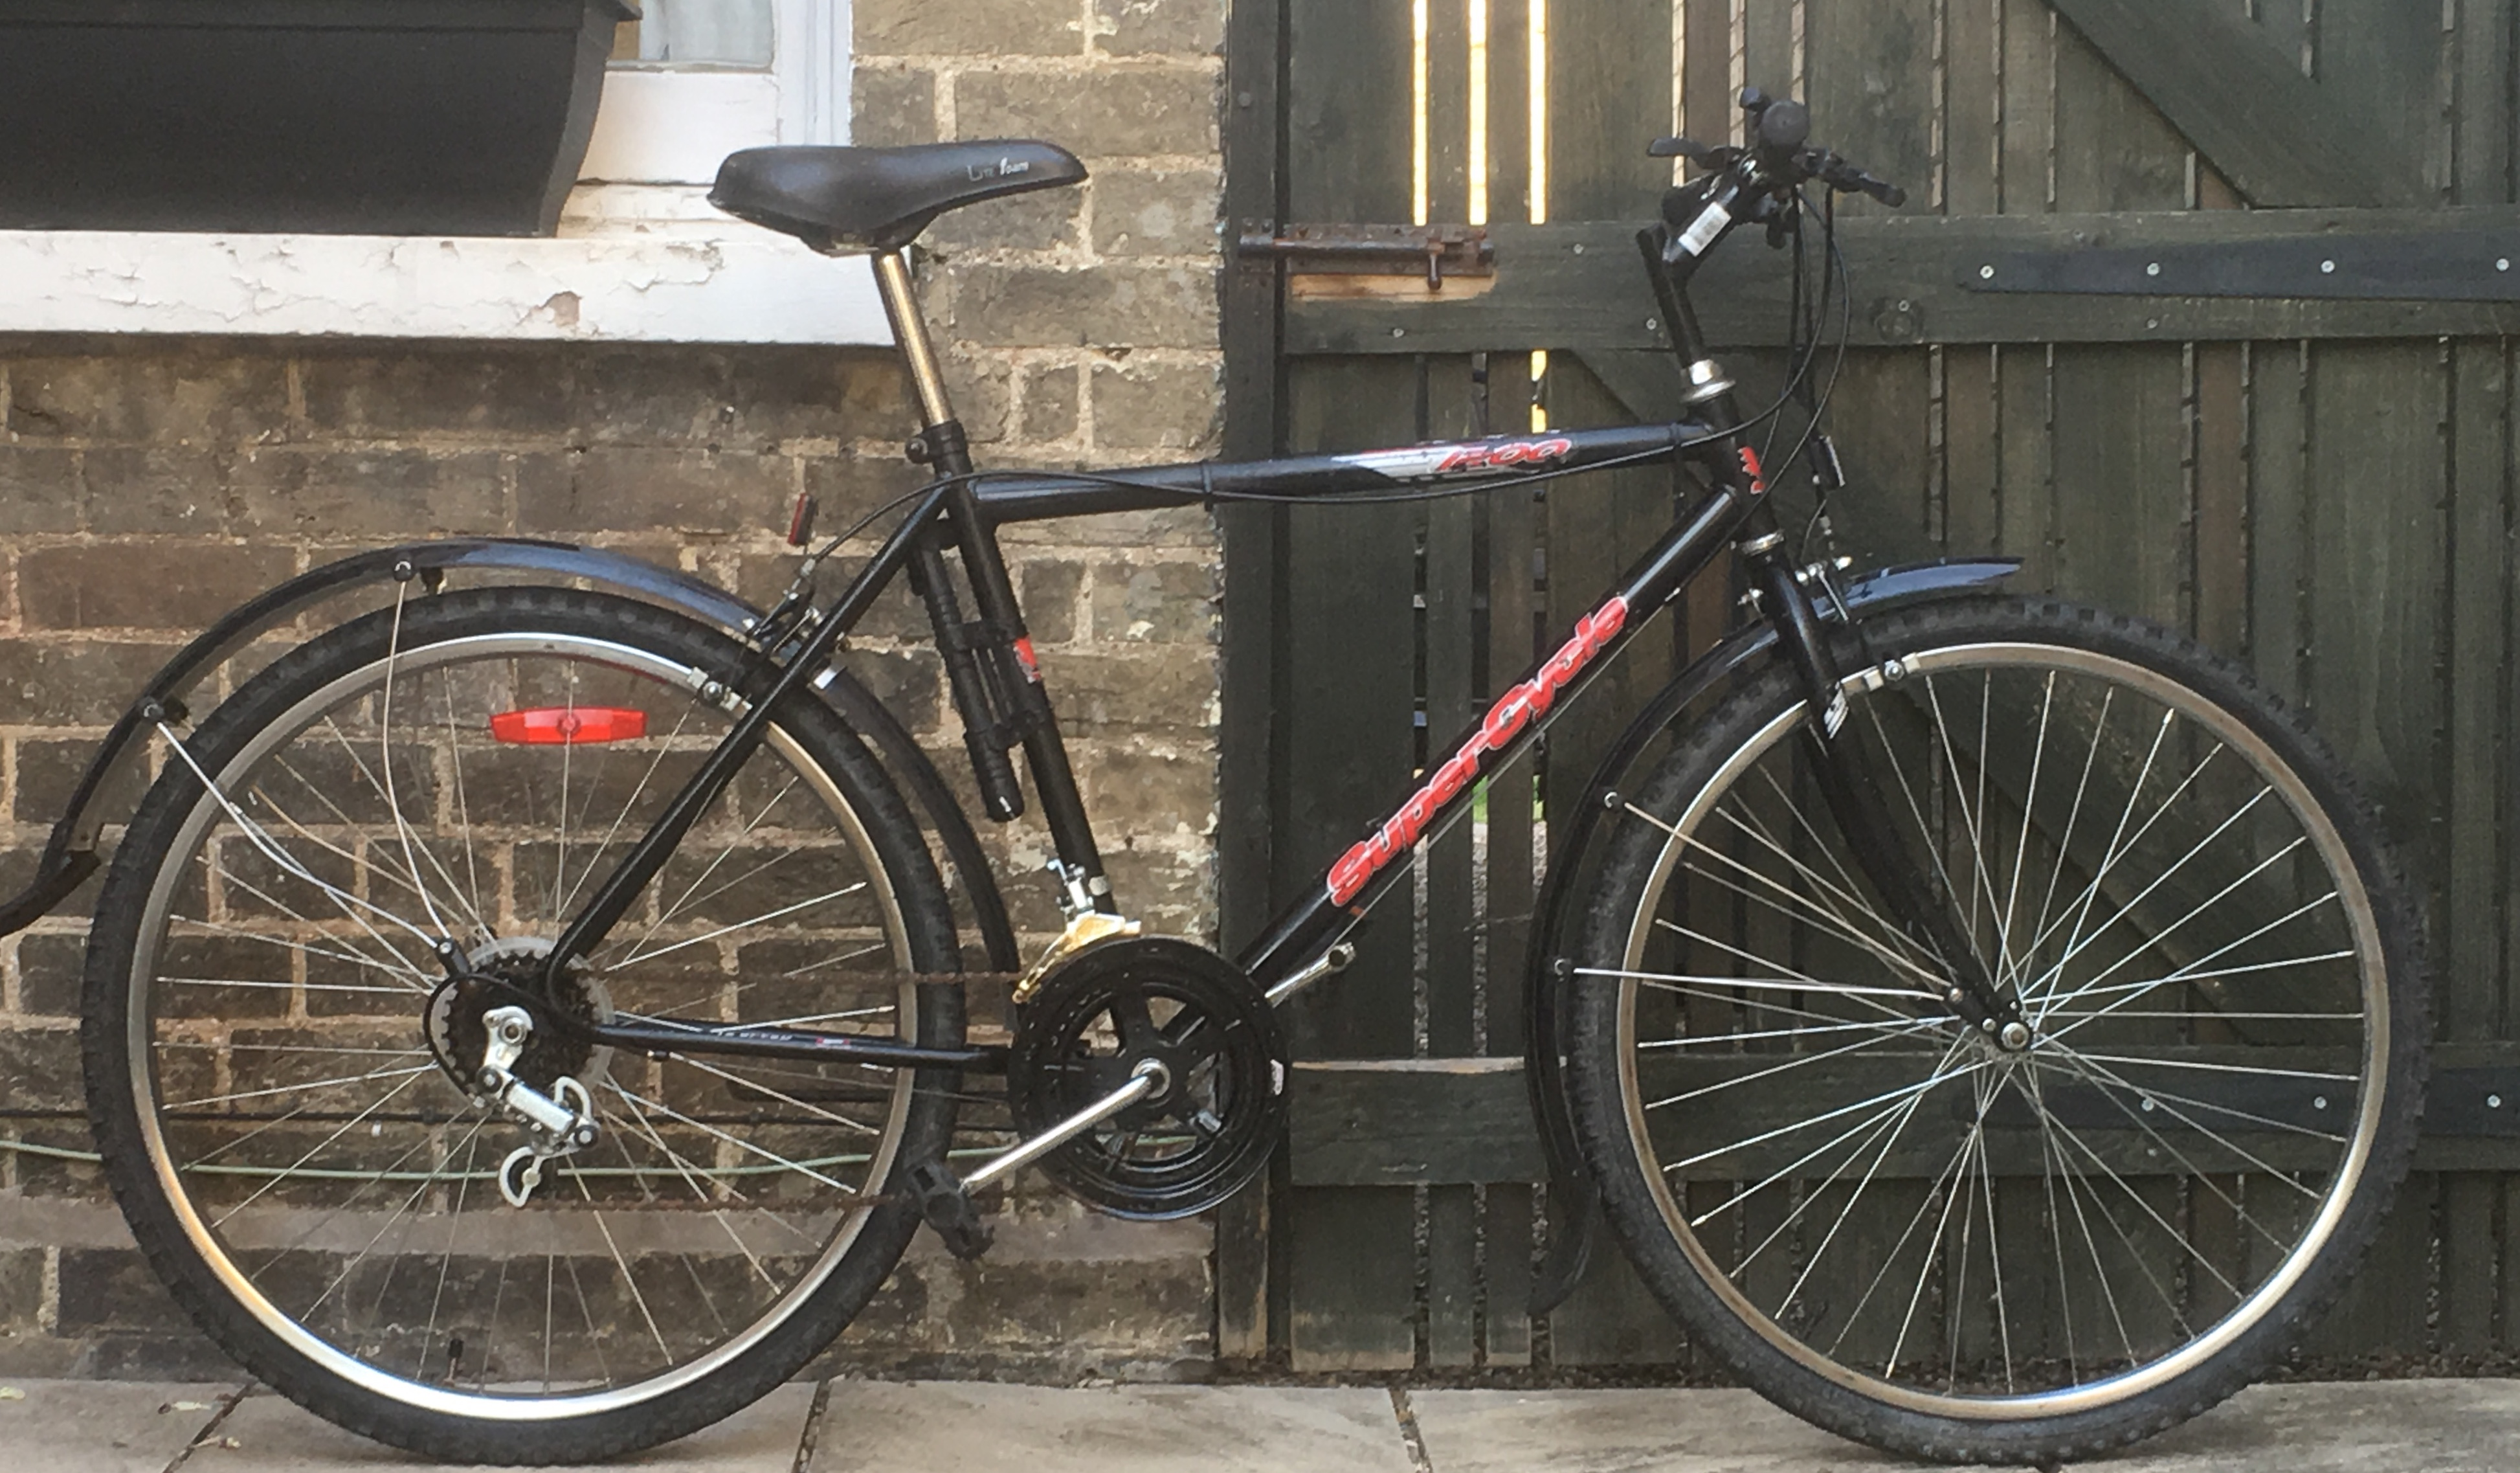
\includegraphics[scale=0.075]{FSBike.jpg}
\caption{Full-Scale Bicycle}
\label{fig:fs}
\end{figure}